%
% Copyright (c) 2017  Zubax Robotics OU  <info@zubax.com>
%
% Distributed under BY-NC-ND (attribution required, non-commercial use only, no derivatives).
%

\documentclass{zubaxdoc}
\graphicspath{{document_templates/documentation_template_latex/}}

\title{Zubax GNSS 2 Datasheet}

\begin{document}
\frontmatter

\begin{titlepage}

\section*{Overview}

Zubax GNSS 2 is a multipurpose high-performance positioning module interfaced via CAN bus, USB, and UART.
It includes a state-of-the-art multi-system GPS/\allowbreak{}GLONASS receiver,
a high-precision barometric altimeter, and a 3-axis compass with thermal compensation.

\section*{Features}

\begin{itemize}
    \item State-of-the-art concurrent GPS/GLONASS receiver u-blox MAX-M8Q.
    \begin{itemize}
    	\item Full RF shielding of the GNSS circuits ensures reliable operation in high-EMI environments.
    	\item 35 mm high-gain patch antenna with large ground plane for reliable reception even in deep urban canyons.
    	\item Analog front-end with LNA and SAW ensures high noise resilience.
    	\item Supercapacitor-based backup power source enables low time-to-first-fix (a few seconds).
    	\item Up to 15 Hz update rate.
    \end{itemize}
	\item High precision digital barometer TE Connectivity MS5611.
    \item High precision 3-axis digital compass STMicroelectronics LIS3MDL with thermal compensation.
	\item Supported interfaces:
    \begin{itemize}
        \item CAN, with optional double redundancy.
        \item UART.
        \item USB port, no drivers needed.
    \end{itemize}
    \item High quality assurance:
    \begin{itemize}
        \item Every manufactured unit undergoes a strict testing procedure.
        The testing log for each produced unit is available to the user via the website at\\
        \url{https://device.zubax.com/device_info}.
        \item Protection against unlicensed (counterfeit) production by means of a digital signature
        installed on every manufactured unit.
    \end{itemize}
\end{itemize}

\BeginRightColumn

\section*{Applications}

\begin{itemize}
	\item Positioning module for unmanned vehicles (aerial, ground, underwater, etc) and robots.
    \item General-purpose embedded positioning module.
\end{itemize}

\centering
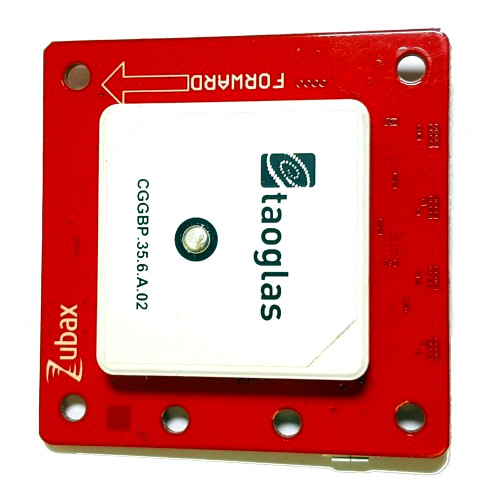
\includegraphics[width=0.45\textwidth]{GNSS_top}
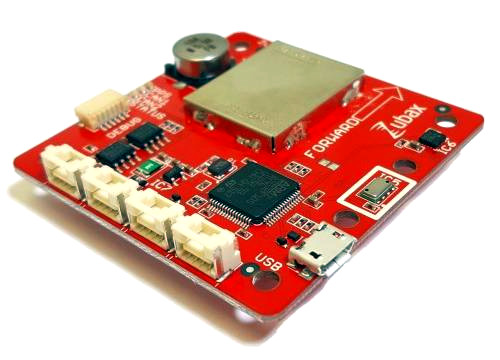
\includegraphics[width=0.45\textwidth]{GNSS_bottom}
\end{titlepage}

\tableofcontents
\BeginRightColumn
\listoffigures
\listoftables

\mainmatter

\chapter{Overview}

Zubax GNSS 2 is a multipurpose high-performance positioning module interfaced via CAN bus, USB, and UART.
It includes a state-of-the-art multi-system GPS/GLONASS receiver, a high-precision barometric altimeter, and a 3-axis compass with thermal compensation.
Zubax GNSS 2 supports a variety of standard protocols, which ensures compatibility with third party software and hardware: UAVCAN (over CAN bus), NMEA 0183 (over USB and UART), and the u-Blox M8 binary protocol.

\section{Quality assurance}

Every manufactured Zubax GNSS 2 undergoes an automated testing procedure that validates that
the device is functioning as designed.
The test log for every manufactured device is available on the web at
\url{https://device.zubax.com/device_info}.
This feature can be used to facilitate traceability of purchased devices and
provide additional safety assurances.

Besides testing, every manufactured device has a digital signature installed,
that can be used as a strong protection against unlicensed or counterfeit manufacturing.
Please contact Zubax Robotics
to find out the specifics about digital signature verification.

\section{Enclosure}\label{sec:enclosure}

Zubax GNSS 2 is intended for integration into the end system in the form of the bare PCB,
as this facilitates lower weight and tighter arrangement of components
in the end device, all of which are desirable properties in the target application domains.

Shall it be desired to provide additional mechanical protection for the device or to install it away from possible sources of electromagnetic interference, the plastic components pictured on the figure \ref{enclosure} can be used.
Please contact your supplier for the ordering information;
alternatively, visit \url{https://github.com/Zubax/zubax_gnss/} to download
the 3D printable enclosure models suitable for in-house manufacturing.

\begin{figure}[hb]
	\centering
	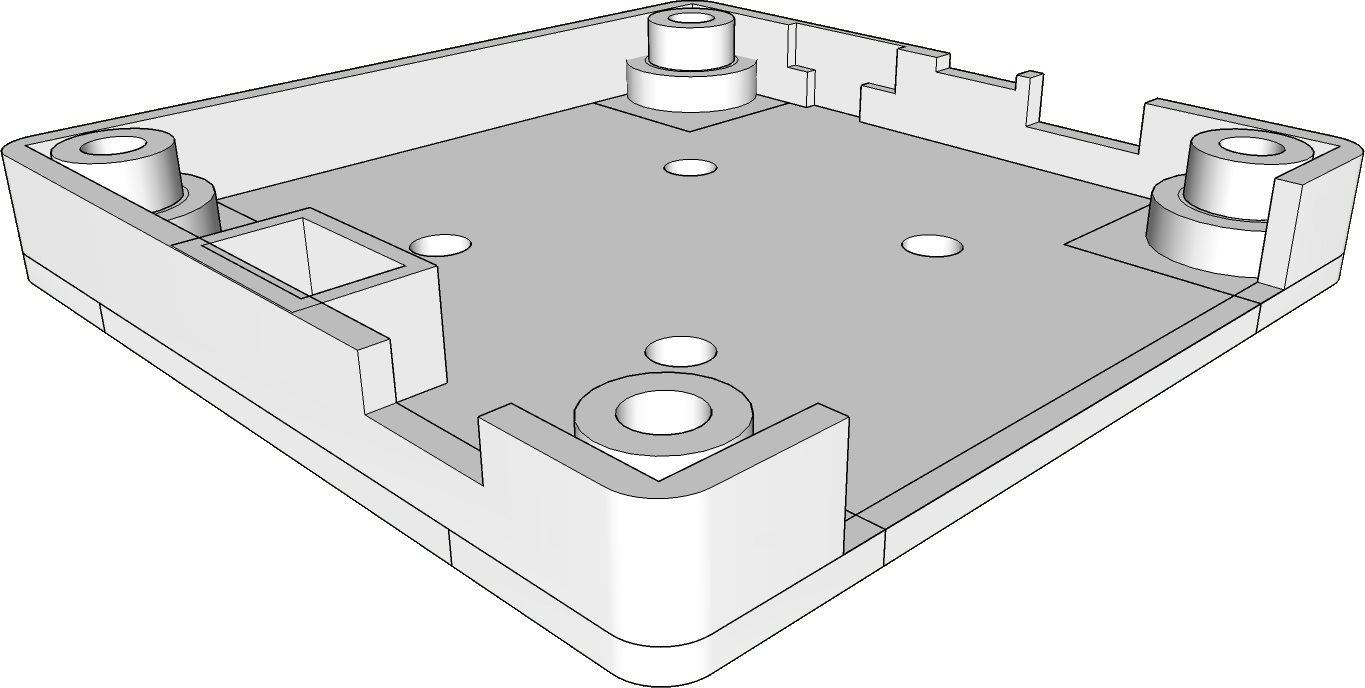
\includegraphics[width=0.45\textwidth]{housing}
	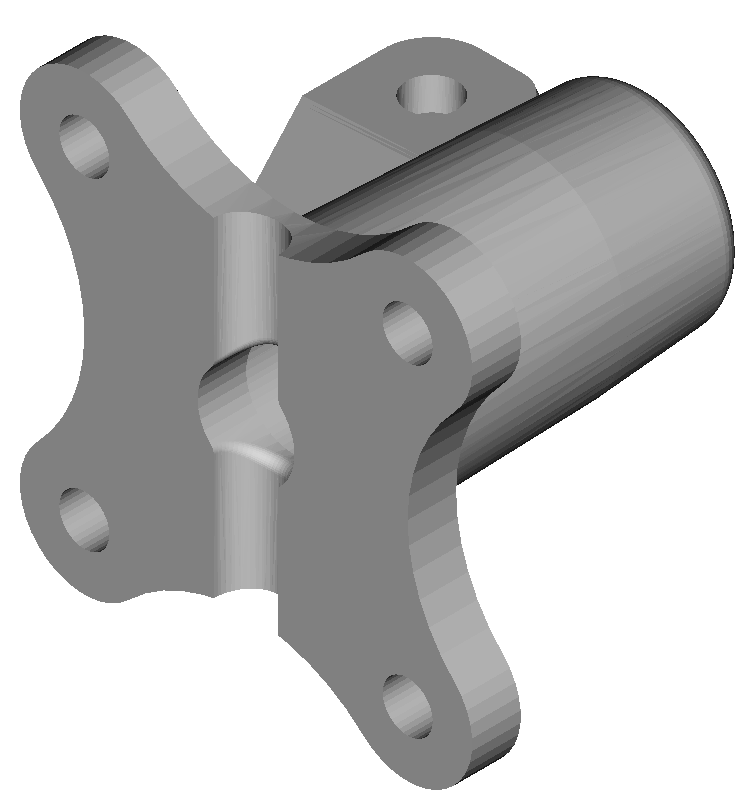
\includegraphics[width=0.45\textwidth]{post}
	\caption{Plastic enclosure and post.\label{enclosure}}
\end{figure}

\section{Accessories}

Zubax GNSS 2 can be used with the following accessories:

\begin{itemize}
    \item Enclosure (suitable for 3D printing). See section \ref{sec:enclosure}.
    \item UAVCAN Micro patch cable.
    \item UAVCAN Micro adapter cables.
    \item UAVCAN Micro termination plug.
    \item Zubax DroneCode Debug Probe.
\end{itemize}

Please contact your supplier for ordering information.

\chapter{Characteristics}

\section{Absolute maximum ratings}

Subjecting the device to stresses beyond those specified in this section may cause
permanent damage to the device.
Proper operation of the device within the ranges specified in this section is not implied.

\begin{ZubaxSimpleTable}{Absolute maximum ratings}{|c X|c c|c|}
    Symbol            & Parameter                & Min  & Max & Unit \\
	$V_\text{inv}$    & Supply voltage           & -0.3 & 6   & V \\
	$T_\text{oper}$   & Operating temperature    & -50  & 125 & \degree{}C \\
	                  & UART input voltage 		& -0.3 & 6   & V\\
	                  & CAN H/L input voltage    & -4   & 16  & V\\
\end{ZubaxSimpleTable}

\section{Environmental conditions}

\begin{ZubaxSimpleTable}{Environmental conditions}{|c |l c|c|c|}
     Parameter &  Min & Max & Unit  & Note \\
	 Board temperature & -40 & 70 & \degree{}C & GNSS hot start is not expected to work reliably below -20\degree{}C	\\
	 Magnetic field strength	&	& 9 &	Gauss & 
\end{ZubaxSimpleTable}

\section{Reliability}

\begin{ZubaxSimpleTable}{Reliability}{|c X|c|c|}
    Symbol & Parameter & Typ & Unit \\
	MTTF   & Mean time to failure & 100000 & hours \\
\end{ZubaxSimpleTable}

\section{Power Supply}

\begin{ZubaxSimpleTable}{Power supply}{|c |c c c | c|X|}
     Parameter &  Min & Typical & Max & Unit  & Note \\
	 Supply voltage & 4.5 & 5.0 & 5.5 & V  & Any power input\\
	 Supply current & 70  & 95  & 180 & mA & Any power input\\
\end{ZubaxSimpleTable}

\section{Communication interfaces}

Zubax GNSS 2 features three communication interfaces, each of which is described in detail in the subsequent parts of this document. The interfaces are as follows:
\begin {itemize}
\item Doubly redundant UAVCAN interface with two connectors for each interface. This interface provides access to all features of Zubax GNSS 2, including measurements output, configuration, time synchronization, firmware update, etc. Connector type is UAVCAN Micro connector (JST GH).
\item USB port (CDC ACM profile, also known as virtual serial port). This interface can be used for NMEA output and configuration. Connector type is USB micro B (which is the most common USB connector).
\item DroneCode port, used for NMEA output and diagnostics. Connector type is DCD-M (JST SH)
\end{itemize}

The device can be powered via the following:
\begin {itemize}
\item Any single UAVCAN port.
\item Both UAVCAN ports simultaneously (the power supply circuit prevents direct current flow between these power inputs).
\item USB
\item DroneCode port (hardware revisions v2.1 and newer).
\end{itemize}

It is allowed to power the device simultaneously via USB and UAVCAN, since the power supply circuit prevents back-powering via these interfaces.

Power supply characteristics are identical regardless of the power input used - refer to the tables below for details.

\begin{ZubaxTableWrapper}{Characteristics of CAN bus interfaces}
	\begin{ZubaxWrappedTable}{|c X|c c c|c|}
		Symbol  & Parameter                                 & Min  & Typ  & Max  & Unit \\
		        & Bit rate                                  & 20   &      & 1000 & Kbps \\
		        & Positive-going input threshold voltage    &      & 750  & 900  & mV \\
		        & Negative-going input threshold voltage    & 500  & 600  &      & mV \\
		        & Differential output voltage, dominant     & 1.5  & 2.0  & 3.0  & V \\
		        & Differential output voltage, recessive    & -120 & 0    & 12   & mV \\
		        & Bus power rail\tnote{1}\space{} voltage   & -10  &      & 10   & V \\
		        & Inter-connector current\tnote{1}          & -1 &  & 1    & A \\
		        & Connector resistance during device lifetime &    & 30   & 50   & $\text{m}\Omega$ \\
	\end{ZubaxWrappedTable}
	\begin{tablenotes}
	    \item [1] The limit is imposed by the PCB.
	\end{tablenotes}
\end{ZubaxTableWrapper}

\subsection{DroneCode debug port}

The device features a DroneCode debug port available via the standard
DroneCode Mini debug connector (DCD-M)\footnote{Refer to the DroneCode documentation
for more information on standard connectors and communication interfaces.}.
The DroneCode debug port provides access to the device's CLI\footnote{Command line interface.}
via UART.

\begin{ZubaxSimpleTable}{DroneCode debug port characteristics}{|c X|c c c|c|}
	Symbol  & Parameter                                 & Min  & Typ  & Max  & Unit \\
			& Low-level input voltage                   & -0.3 & 0    & 1.6  & V\\
			& High-level input voltage                  & 2.1  & 3.3  & 5.5  & V\\
			& Low-level output voltage                  & 0    & 0    & 0.5  & V\\
			& High-level output voltage                 & 2.8  & 3.3  & 3.4  & V\\
			& Source/sink current via data pins         &      &      & 10   & mA\\
			& UART RX 							       & 15   & 20   & 25   & $\text{k}\Omega$\\
	$V_\text{DCDP}$ & Power rail output voltage         & 3.2  & 3.3  & 3.4  & V\\
	$I_\text{DCDP}$ & Power rail load capability        &      &      & 3    & mA\\
	        & Connector resistance during device lifetime &    & 20   & 40   & $\text{m}\Omega$\\
\end{ZubaxSimpleTable}

\chapter{LED Indication}

\section{PPS LED}

This LED indicator blinks with the rate of 1 Hz if the GNSS receiver has a navigation fix.

\section{Status LED}

This LED indicator shows the health of the device derived from the continuous self-diagnostics as described above:

\begin{ZubaxSimpleTable}{Status LED indication}{|X|X|}
Health 	& Blinking ON/OFF duration \\
OK		& 0.05/0.95 seconds\\
WARNING	& 0.05/0.25 seconds\\
ERROR	& 0.05/0.05 seconds
\end{ZubaxSimpleTable}

\section{CAN1 and CAN2 LEDs}

These LED indicators show the CAN bus traffic.

Each blink indicates that there was a CAN frame that was successfully transmitted or successfully received during the last few milliseconds. Under high bus load, these LED indicators are expected to glow steadily. If the interface is not connected to the bus, its LED indicator will be inactive, even if the device is actually attempting to transmit.

Note that CAN frames filtered out by the hardware acceptance filters will not cause the LED indicators to blink.

\section{LED indication during firmware update and bootup}

\subsection{Firmware v4.0 and newer}

During first few seconds after power-on or after restart, and also in the process of firmware update, Zubax GNSS 2 uses its LED indicators in a different way, as described in the section dedicated to the bootloader below.
\subsection{Firmware v3.x and older}

During first few seconds after power-on or after restart, and also in the process of firmware update, Zubax GNSS 2 uses its LED indicators in a different way, as described in the table below.

\begin{ZubaxSimpleTable}{CAN LED indication at bootup}{| X | c | c | c|}
Status & INFO & CAN1 & CAN2 \\
CAN bit rate detection &  & Solid & \\
Dynamic node ID allocation & Solid & &  \\
Update in progress & Solid & Solid & \\
\end{ZubaxSimpleTable}

\chapter{UAVCAN interface}

This section describes the properties specific for this product only. For general info about the UAVCAN interface, please refer to the UAVCAN interface documentation page.

If Zubax GNSS 2 is used in a setup with non-redundant CAN bus, only CAN1 must be used.

\section{Mode and status codes}

Zubax GNSS 2 employs the following UAVCAN-defined operating modes:

\begin{ZubaxSimpleTable}{UAVCAN-defined operating modes}{|c|X|}
UAVCAN operating mode & Conditions\\
INITIALIZING		& The device has just started and is not ready to begin normal operation yet.\\
OPERATIONAL	& This is the main operating mode.\\
SOFTWARE UPDATE	& The device is undergoing firmware update via UAVCAN. It will automatically transition to OPERATIONAL mode upon completion.
\end{ZubaxSimpleTable}

While the device resides in OPERATIONAL mode, its internal health codes are mapped directly to UAVCAN health codes. The description of internal health codes is provided above.

The following table describes the meanings of the standard UAVCAN health codes in the mode SOFTWARE\_UPDATE.

\begin{ZubaxSimpleTable}{UAVCAN-defined operating modes}{|c|X|}
UAVCAN health code & Possible reasons\\
OK 		& 	Everything is OK.\\
WARNING	& Not used.\\
ERROR 	& Not used.\\
CRITICAL & Firmware update has failed; another attempt will be made soon
\end{ZubaxSimpleTable}

\section{Time synchronization}

This device can act as a UAVCAN-compliant time synchronization master, but this feature is disabled by default. If time synchronization is enabled, the GNSS UTC time will be used as the time source, which implies that the time synchronization master will be functional only if the device has had at least one successful GNSS time fix since power on.
\clearpage 

\section{Services}

This device does not call any services.

The following service servers are implemented:

\begin{ZubaxSimpleTable}{UAVCAN services}{|l|X|}
Data type & Note \\
\texttt{uavcan.protocol.GetNodeInfo} & Please refer to the identification information section. \\
\texttt{uavcan.protocol.GetDataTypeInfo}& \\
\texttt{uavcan.protocol.GetTransportStats} & \\
\texttt{uavcan.protocol.RestartNode} & \\
\texttt{uavcan.protocol.file.BeginFirmwareUpdate} & Reboots the device into the bootloader and commences the firmware download process.\\
\texttt{uavcan.protocol.param.GetSet} & Configuration parameters are described in this document below .\\
\texttt{uavcan.protocol.param.ExecuteOpcode} & Note that this request may cause transient disruptions to output sensor feeds. Starting from firmware v4.0, configuration parameters are saved automatically after modification, so no explicit invocation of this service is necessary.
\end{ZubaxSimpleTable}
\clearpage

\section{Messages}

\begin{ZubaxSimpleTable}{Input Messages}{|l|X|}
Data type & Note \\
\texttt{uavcan.protocol.GlobalTimeSync} & Always synchronizes with network time, if present. \\
\texttt{uavcan.protocol.dynamic{\_}node{\_}id.Allocation} & Used to allocate node ID if dynamic node ID allocation is enabled (it is enabled by default).
\end{ZubaxSimpleTable}

\begin{ZubaxSimpleTable}{Output Messages}{|X|X|}
Data type & Note \\
\texttt{uavcan.protocol.GlobalTimeSync} & Disabled by default.\\
\texttt{uavcan.protocol.NodeStatus} &  \\
\texttt{uavcan.equipment.gnss.Fix} & This message definition is deprecated; refer to the UAVCAN specification for detail. Enabled by default for compatibility reasons, but \textbf{it is recommended to disable it}.\\
\texttt{uavcan.equipment.gnss.Fix2} & This is a replacement to the deprecated message type \texttt{uavcan.equipment.gnss.Fix}.\\
\texttt{uavcan.equipment.gnss.Auxiliary} & \\
\texttt{uavcan.equipment.ahrs.MagneticFieldStrength} & \\
\texttt{uavcan.equipment.air{\_}data.StaticPressure} & Disabled by default.\\
\texttt{uavcan.equipment.air{\_}data.StaticTemperature} & Priority is shared with 
\texttt{uavcan.equipment.air{\_}data.StaticPressure}  See a note below on publication frequency. Disabled by default.\\
\texttt{uavcan.protocol.dynamic{\_}node{\_}id.Allocation} & Used to allocate node ID if dynamic node ID allocation is enabled (it is enabled by default).
\end{ZubaxSimpleTable}

The publication frequency of \texttt{uavcan.equipment.air{\_}data.StaticTemperature} is defined as follows:
\begin{itemize}
\item For firmware versions prior to v4.0, the message \texttt{uavcan.equipment.air{\_}data.StaticTemperature} is published at the same rate as \texttt{uavcan.equipment.air{\_}data.StaticPressure}.
\item For firmware versions v4.0 and newer, the message \texttt{uavcan.equipment.air{\_}data.StaticTemperature} is published at 1/5th of the rate of \texttt{uavcan.equipment.air{\_}data.StaticPressure}. E.g. if the pressure data is broadcasted at 20 Hz, the temperature data will be broadcasted at 4 Hz.
\end{itemize}

\chapter{USB interface}

The USB interface allows to use Zubax GNSS 2 as a standalone USB GNSS receiver (also known as ''GPS mouse'') interfaced via the standard NMEA 0183 protocol; also it provides access to configuration parameters.

\section{Protocol selection}

Zubax GNSS 2 will automatically enable NMEA output via USB if the virtual serial port is opened with any baud rate within the range 4800 to 57600 baud, inclusive. If the port is open with any other baud rate, e.g. 115200, NMEA output will not be enabled, and only the command line interface will be available.
 
The baud rate range is chosen this way because all standard NMEA baud rates fall within this range, which allows to use Zubax GNSS 2 with GNSS software (e.g. GIS systems, navigation software, etc.) right out of the box without any preparatory configuration.

\section{NMEA output}

Zubax GNSS 2 reports sensor data using the following standard NMEA sentences. Please also refer to the list of configuration parameters below to see what can be adjusted if necessary.

More information on NMEA can be found here: \href{http://www.catb.org/gpsd/NMEA.html}{http://www.catb.org/gpsd/NMEA.html}.

Refer to the tutorials to see examples of using Zubax GNSS 2 with GIS software.

\begin{ZubaxSimpleTable}{Input Messages}{|l|c|X|}
NMEA sentence & Component & Purpose\\
\texttt{GPRMS} & GNSS receiver & Recommended minimum navigation information.\\
\texttt{GPGGA} & GNSS receiver & Global positioning system fix data.\\
\texttt{GPGSA} & GNSS receiver & GPS DOP and active satellites.\\
\texttt{GPGSV} & GNSS receiver & Information about satellites in view.\\
\texttt{HCHDG} &	 Compass		  & Raw magnetic heading; not calibrated, only valid if the board is mounted horizontally.\\
\texttt{YXXDR} (type P) & Altimeter & Static barometric pressure (only if the sensor is enabled).\\
\texttt{YXXDR} (type C) & Altimeter & Static air temperature (only if the sensor is enabled).
\end{ZubaxSimpleTable}
\clearpage

\subsection{Vendor-specific sentences}

The NMEA specification dedicates the prefix {\$}P followed by the vendor ID for vendor-specific sentences. All Zubax products use the vendor-specific prefix ZUBAX. The first field of the sentence contains the sentence type identifier, which is a string containing upper case Latin letters, Arabic digits, and the minus symbol -.

\subsubsection{Raw magnetic field strength}

Vendor-specific sentence type ID: \textbf{MAG-FLD-XYZ}.

Availability: firmware v4.0 and newer.

Fields:

\begin{enumerate}
\item Magnetic field strength of the X axis.
\item Magnetic field strength of the Y axis.
\item Magnetic field strength of the Z axis.
\item A single character \texttt{G} that indicates that the units of measurement are Gauss.
\item Reserved.
\item Reserved.
\end{enumerate}

Example: \verb|PZUBAX,MAG-FLD-XYZ,1.345,-1.345,0.345,G,,*12|.

\subsection{Sample output}

\begin{minted}[linenos = false]{text}
$GPRMC,072626.30,A,0036.27144,N,00042.93538,E,1.097,235.8,141215,,*35
$GPGGA,072626.30,0036.27144,N,00042.93538,E,1,14,1.44,239.382,M,13.2,M,,*5E
$GPGSV,4,1,15,08,52,283,17,10,80,126,26,14,27,155,34,15,15,039,08*74
$GPGSV,4,2,15,16,00,216,16,18,49,073,13,21,25,109,22,22,77,181,25*7F
$GPGSV,4,3,15,27,59,219,15,32,03,232,16,01,74,188,27,02,19,214,17*76
$GPGSV,4,4,15,08,47,047,22,23,29,145,21,24,80,177,18*4A
$HCHDG,266.0,,,,*40
$YXXDR,P,0.98966,B*57
$YXXDR,C,29.9,C*7F
$GPRMC,072626.36,A,0036.27143,N,00042.93547,E,1.402,235.8,141215,,*34
$GPGGA,072626.36,0036.27143,N,00042.93547,E,1,15,1.44,239.467,M,13.2,M,,*5A
$GPGSA,A,3,08,10,14,18,21,22,27,01,02,23,24,12,2.24,1.44,1.71*04
$HCHDG,266.2,,,,*42
$YXXDR,P,0.98968,B*59
\end{minted}
\clearpage

\section{Command-line interface}

This section documents supported CLI commands.

\textbf{zubax{\_}id}

This is the standard Zubax identification command. It is supported by all devices that implement a command line interface. Please refer to the USB command line interface documentation page for more info.

\textbf{cfg}

Allows to view or modify configuration parameters.
Execute without arguments to get usage info. Supported arguments:
\begin{itemize}
\item \textbf{list} - list all parameters, their values and ranges.
\item \textbf{set <name> <value>} - change parameter value.
\item \textbf{save} - save all parameters to the non-volatile memory (see the note).
\item \textbf{erase} - reset all parameters to defaults.
\end{itemize}

Starting from firmware v4.0, configuration parameters are saved automatically after modification. Thus, it is no longer necessary to execute \textbf{cfg save}.

\textbf{reset}

Restarts the device. Note that sensors will not be restarted.

\textbf{gnssbridge}

Activates the direct bridge connection between USB CLI and the GNSS receiver. This feature allows to receive GNSS information using native u-Blox M8 protocol.

Once the bridge is activated, the state of the device changes as follows until reboot:
\begin{itemize}
\item CLI becomes unavailable because it is being used to communicate with the GNSS receiver.
\item The device stops publishing GNSS messages via UAVCAN.
\item Status code changes to CRITICAL because GNSS sensor data are not available anymore.
\end{itemize}

Aside from the above, the device continues to work virtually as usual, e.g., its UAVCAN stack operates normally, other sensors are working (if enabled), etc.

\textbf{help}

Prints the list of available commands

\textbf{bootloader}

Available in firmware v4.0+.

Reboots the board into the bootloader.

\chapter{DroneCode port}

DroneCode port provides access to JTAG/SWD and UART interfaces. This port allows to update firmware and provides access to the UART interface that is used to log events, report problems, and output measurements in NMEA format. Hardware revisions v2.1 and newer can also be powered via this port.

DroneCode port can be accessed using \href{https://kb.zubax.com/display/MAINKB/Dronecode+Probe+documentation}{Zubax DroneCode Probe}.

If outputting NMEA over UART is not of interest, this port will not be needed during normal use of the device.

\section{NMEA output over UART}

For general information about NMEA output interface, refer to the corresponding section above. Note that NMEA output over UART is disabled by default; refer to the description of configuration parameters to see how to enable it.

The following connector pinout can be used to read NMEA over UART:

\begin{ZubaxSimpleTable}{DroneCode Mini debug connector pinout}{| c | c | c | X |}
	Pin & Type  & Name                & Comment \\
	1   & Power & +5VDC               & Power supply (hardware v2.1 and newer). On hardware v2.0 this pin must be left unconnected.\\
	2 	& OUT	& UART{\_}TX			& NMEA output\\
	3 & N/C & & \\
	4 & N/C & & \\
	5 & N/C & & \\
	6 & GND & GND & Ground \\
\end{ZubaxSimpleTable}

UART parameters are fixed and provided below:
\begin{itemize}
\item Baud rate: 115200
\item Byte size: 8
\item Parity: None
\item Stop bits: 1
\end{itemize}

\chapter{Configuration parameters}

This section documents the available configuration parameters. Read the documentation on the interfaces to learn how to access the configuration parameters.

Reboot is required in order for all configuration changes to take effect.

Starting from firmware v4.0, configuration parameters are saved automatically after modification.

\textbf{uavcan.bit{\_}rate}

Removed in firmware v4.0.

CAN bus bit rate, all interfaces. Value 0 (which is default) causes the device to detect bit rate automatically at every boot up.

Default value: 0

Units: bits/sec

\textbf{uavcan.node{\_}id}

UAVCAN Node ID Value 0 (which is default) causes the device to request a dynamically allocated node ID at every boot up.

Default value: 0

\textbf{uavcan.pubp-time}

Publication interval of \texttt{uavcan.protocol.GlobalTimeSync}. Zero means disabled.

Default value: 0

Units: Microsecond

\textbf{uavcan.prio-stat}

Priority of \texttt{uavcan.protocol.NodeStatus}.

Default value: 20

\textbf{uavcan.pubp-pres}

Publication interval of \texttt{uavcan.equipment.air{\_}data.StaticPressure}. Zero means disabled. When disabled:
\begin{itemize}
\item The driver of the appropriate sensor will not be initialized.
\item The sensor will not be monitored - implying that, if it fails, it will not be detected and reported.
\item Measurements will not be reported via any of the available interfaces.
\end{itemize}
This setting also affects \texttt{uavcan.equipment.air{\_}data.StaticPressure}.

Default value: 0 (disabled)

Units: Microsecond

\textbf{uavcan.prio-pres}

Priority of \texttt{uavcan.equipment.air{\_}data.StaticPressure}. This setting also affects \texttt{uavcan.equipment.air{\_}data.StaticPressure}.

Default value: 16
 
\textbf{uavcan.pubp-mag}

Publication interval of \texttt{uavcan.equipment.ahrs.MagneticFieldStrength}.

Default value: 20000

Units: Microsecond

\textbf{uavcan.prio-mag}

Priority of \texttt{uavcan.equipment.ahrs.MagneticFieldStrength}.

Default value: 16

\textbf{uavcan.pubp-fix}

Publication interval of \texttt{uavcan.equipment.gnss.Fix}.

Default value: 100000

Units: Microsecond

\textbf{uavcan.pubp-aux}

Publication interval of \texttt{uavcan.equipment.gnss.Auxiliary}.

Default value: 1000000

Units: Microsecond

\textbf{uavcan.prio-fix}

Firmware v4.0 and newer

This setting directly assigns the priority of the message \texttt{uavcan.equipment.gnss.Fix2}. The deprecated message  \texttt{uavcan.equipment.gnss.Fix}, if enabled, will be using the next lower priority level. For example, if this setting is set to 16, the deprecated message will be broadcasted at the priority level 17, which is one lower than 16.

Default value: 16

Firmware v3.x and older

Priority of \texttt{uavcan.equipment.gnss.Fix}.

Default value: 16

\textbf{uavcan.prio-aux}

Priority of \texttt{uavcan.equipment.gnss.Auxiliary}.

Default value: 20

\textbf{pres.variance}

Pressure variance reported via \texttt{uavcan.equipment.air{\_}data.StaticAirData}.

Default value: 100

Units: $\text{Pascal}^2$

\textbf{temp.variance}

Temperature variance reported via \texttt{uavcan.equipment.air{\_}data.StaticAirData}.

Default value: 4

Units: $\text{Kelvin}^2$

\textbf{mag.variance}

Magnetic field variance reported via \texttt{uavcan.equipment.ahrs.Magnetometer}.

Default value: 0.005

Units: $\text{Gauss}^2$

\textbf{mag.scaling{\_}coef}

New in firmware v3.1.

Magnetic field vector scale. Some UAV autopilot systems (PX4, APM) do not correctly handle magnetic field measurements made in highly magnetically distorted environments. It is possible to work around these issues by reducing the magnitude of the magnetic field vector.

For PX4 and APM users: if your autopilot reports that magnetometer offsets are too high, reduce this parameter to approximately 0.6 and recalibrate the magnetometer.

Default value: 1.0, i.e. no rescaling.

\textbf{gnss.warn{\_}dimens}

Set the node status to WARNING if the number of dimensions in the GNSS solution is below this threshold. Values: 1 - time-only fix, 2 - 2D fix, 3 - 3D fix.

Default value: 0

\textbf{gnss.warn{\_}sats}

Set the node status to WARNING if the number of satellites used in the GNSS solution is below this threshold.

Default value: 0

\textbf{nmea.uart{\_}on}

Enable NMEA output via DroneCode port (UART). This configuration parameter does not affect NMEA output over USB.

Default value: 0 (disabled)

\textbf{mag.pwron{\_}slftst}

New in firmware v4.0.

Perform power on self test of the magnetometer when booting. Note that the manufacturer of the magnetometer recommends to hold the sensor stationary during the self test procedure. Therefore it is recommended to disable this feature unless it is expected that the board will be always held stationary during powering on. Otherwise the self test may be occasionally failing, delaying the proper start up of the device.

Default value: 1 (enabled)

\textbf{gnss.old{\_}fix{\_}msg}

New in firmware v4.0.

Broadcast the deprecated message \texttt{uavcan.equipment.gnss.Fix} alongside the new message\\ \texttt{uavcan.equipment.gnss.Fix2}.\\This feature is enabled by default for compatibility purposes; however, it is recommended to disable it in order to reduce the CAN bus traffic if it is not needed.

Default value: 1 (compatibility mode)

\chapter{Identification information}

This section documents the device properties that are reported in response to identification requests: the CLI command \textbf{zubax{\_}id} and the UAVCAN service \texttt{uavcan.protocol.GetNodeInfo}.
\begin{itemize}
\item Product ID and UAVCAN node name: \textbf{com.zubax.gnss}.
\item Hardware version: 2.x.
\end{itemize}

\chapter{Firmware update}

Instructions below are only applicable to Zubax GNSS v2.2 and newer. It is recommended to use Zubax Toolbox or the UAVCAN GUI Tool for updating the firmware.

Zubax GNSS 2 employs the Zubax Embedded Bootloader for purposes of firmware update and integrity checking. The following state machine lies at the core of the bootloader.

\begin{figure}[!hbt]
	\centerline{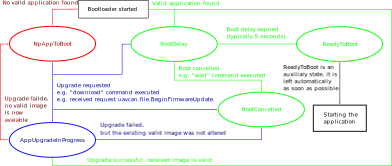
\includegraphics[width=1.1\textwidth]{bootloader_state_machine}}
	\caption{Bootloader state machine.\label{bootloader_state_machine}}
\end{figure}

\begin{ZubaxSimpleTable}{Bootloader states}{|c | l | X|}
State ID & State name & Comment \\
0 & NoAppToBoot & There is no valid application to boot; the bootloader will be waiting for commands forever.\\
1 & BootDelay & The bootloader will start the application in a few seconds, unless the boot is cancelled or a firmware update is requested.\\
2 & BootCancelled & There is a valid application to boot, however, boot was cancelled by an external command.\\
3 & AppUpgradeinProgress & Application is currently being upgraded. If interrupted, the bootloader will go into either \textbf{NoAppToBoot} or \textbf{BootCancelled}.\\
4 & ReadyToBoot & The application is about to boot. This state is very transient and is left automatically as soon as possible.
\end{ZubaxSimpleTable}
\clearpage
On Zubax GNSS 2, the boot delay is set to 5 seconds.
The bootloader supports the following communication interfaces:

\begin{ZubaxSimpleTable}{Bootloader communication interfaces}{| l | l | X | X |}
Intreface & Parameters & Protocol & Note\\
USB & CDC ACM & YMODEM, XMODEM, XMODEM-1K (autodetect) & When connected, the DCD port is inactive\\
DCD port (UART) & 115200-8N1(fixed) & Same as USB CDC ACM & Available only while USB is disconnected\\
CAN1 bus & Autoconfigured & UAVCAN firmware update protocol & Always available on CAN1. CAN2 is not used in the bootloader.
\end{ZubaxSimpleTable}

As can be seen from the table, there are two families of protocols: serial and CAN based; both are reviewed below.

\section{Error codes}

The table below provides definitions for the well defined error codes that can be reported by the bootloader.

\begin{ZubaxSimpleTable}{Error codes}{| l | X |}
0 & Success.\\
1 & Unknown error.\\
9001 & Application ROM driver error: erase failed.\\
9002 & Application ROM driver error: write failed.\\
10001 & The current state of the bootloader does not permit the requested operation.\\
10002 & Application image is too large for the device. Download has been aborted.\\
10003 & Failed to write the next downloaded chunk of the application image into the ROM.\\
20001 & X/YMODEM interface write has timed out.\\
20002 & X/YMODEM retries exhausted.\\
20003 & X/YMODEM protocol error.\\
20004 & X/YMODEM transfer has been cancelled by the remote.\\
20005 & X/YMODEM remote has refused to provide the file.\\
30001 & UAVCAN service request has timed out.\\
30002 & UAVCAN file downloading has been interrupted.\\
32767 & Unknown error.
\end{ZubaxSimpleTable}
\clearpage

\section{LED indication}

While the bootloader is running, the LED indicators behave as follows:
\begin{itemize}
\item The status LED is always on, which is the main indicator that the bootloader, rather than the firmware, is currently running
\item The CAN1 LED behaves normally as a CAN bus activity and load indicator, blinking once for 25 milliseconds every time the CAN1 controller successfully transmits or receives a CAN frame.
\item The CAN2 LED displays one of the blinking patterns shown below, depending on which state the bootloader is in. While the bootloader is running, the state of this LED has no relation to the state of the redundant CAN interface (which is CAN2), since the bootloader makes no use of it.
\end{itemize}

\begin{ZubaxSimpleTable}{LED patterns during bootloader stage}{| l | X |}
Bootloader state & LED blinking pattern (step 50 ms) \\
NoAppToBoot  & 10 Hz (very quickly)\\
BootDelay, ReadyToBoot  & Turned off\\
BootCancelled &  1 Hz, short pulses (50 ms)\\
AppUpgradeInProgress & 1 Hz, long pulses (500 ms)
\end{ZubaxSimpleTable}

\section{Via USB/UART}

Once started, the bootloader exposes a CLI via either DCD port or USB. The USB is always preferred if it is connected to the host; otherwise the CLI falls back to the UART interface of the DCD port.

The CLI can be used to query the state of the bootloader, modify it, obtain the information about the running firmware, and upgrade it if necessary.

The CLI prompt is of the following format: \textbf{StateName>}, which features the human readable name of the current state of the bootloader, followed by the ASCII greater character (ASCII code 62), followed by a space. For example:  \textbf{BootDelay>}. Such prompt allows the user (or software) to easily identify the state of the bootloader.

\subsection{CLI commands}

\textbf{reboot}

Restarts the bootloader.

\textbf{zubax{\_}id}

This is the standard command supported by all products by Zubax Robotics that have a CLI. It takes no arguments, and outputs a YAML key-value dictionary containing the vital information about the device, the firmware it is running, unique ID, installed certificates of authenticity, version of the hardware, and possibly some other information. Aside from the standard fields, this command also provides at least the following fields in its output:

\begin{itemize}
\item \textbf{bl{\_}version} - bootloader version, major and minor.
\item \textbf{bl{\_}vcs{\_}commit} - build identifier of the bootloader.
\item \textbf{mode} - set to the string \textbf{bootloader} to indicate that the bootloader is running.
\end{itemize}

If there is a valid firmware, its version information will also be provided via the standard fields \textbf{fw{\_}version} and  \textbf{fw{\_}vcs{\_}commit}. If the bootloader could not find a valid firmware, these fields will be omitted.

\textbf{wait}

Do not boot the application. If the current state is \textbf{BootDelay}, the state will be switched to \textbf{BootCancelled}. In all other states the command will have no effect.

\textbf{download}

Start the serial receiver and prepare to receive the new firmware image as a flat binary via the serial link using either YMODEM, XMODEM, or XMODEM-1K. The bootloader will automatically detect which protocol to use. According to the YMODEM specification, if no transfer was initiated by the host within one minute, the command will exit with an error. Possible error codes are defined in the table above.

Note that while this command is running, the CLI will be unavailable, since the same serial link will be temporarily occupied by the file transfer protocol.

If the YMODEM protocol is used, the file name field in the transfer header packet will be ignored.

There are heaps of software products and scripts that support these file transfer protocols. For instance, the popular program \textbf{sz} (available on most Linux distributions) can be used as follows:
\begin{minted}[linenos = false]{bash}
sz -vv --ymodem --1k \$file > \$port < \$port
\end{minted}

\section{Via CAN bus}

The bootloader supports the UAVCAN firmware update protocol. Please refer to the UAVCAN specification for theory.

The bootloader only utilizes the primary CAN interface, which is CAN1. The redundant interface CAN2 remains in the passive mode while the bootloader is running. It is therefore required that if there is only one interface in use, it must be CAN1.

The following table describes the mapping from the bootloader states to the UAVCAN node status codes:

\begin{ZubaxSimpleTable}{Bootloader states and UAVCAN node status codes}{| X | X | X |}
Bootloader state & UAVCAN node mode & UAVCAN node health\\
NoAppToBoot & SOFTWARE{\_}UPDATE & ERROR\\
BootDelay, ReadyToBoot & MAINTENANCE & OK\\
BootCancelled & MAINTENANCE & WARNING\\
AppUpgradeInProgress & SOFTWARE{\_}UPDATE & OK
\end{ZubaxSimpleTable}

The vendor specific status code of the node status message contains the status code of the last attempt to upgrade the firmware. Please refer to the error code table provided above.
\clearpage

\subsection{Supported messages}
\begin{ZubaxSimpleTable}{Supported messages}{| l | l | l | l |}
Data type & Direction & Period & Transfer priority \\
\texttt{uavcan.protocol.NodeStatus} & Output & 1 Hz & 24(low) \\
\texttt{uavcan.protocol.debug.LogMessage} & Output & Aperiodic & 31(lowest) \\
\texttt{uavcan.protocol.dynamic{\_}node{\_}id.Allocation} & Input/Output & Aperiodic & 24 (low)
\end{ZubaxSimpleTable}

\begin{ZubaxSimpleTable}{Supported messages annotation}{| l | X |}
Data type & Note\\
\texttt{uavcan.protocol.NodeStatus} & Refer to the bootloader state mapping table.\\
\texttt{uavcan.protocol.debug.LogMessage} & Used to report the application upgrade progress and status in a human readable form.\\
\texttt{uavcan.protocol.dynamic{\_}node{\_}id.Allocation} & Used only during initialization, if the application did not provide a specific node ID to use.
\end{ZubaxSimpleTable}
\clearpage

\subsection{Supported services}

\begin{ZubaxSimpleTable}{Supported servers}{| l | X |}
Data type & Note\\
uavcan.protocol.GetNodeInfo & The nested structure  \textbf{uavcan.protocol.SoftwareVersion} is populated only if there is a valid application.\\
uavcan.protocol.RestartNode & Restarts the bootloader.\\
uavcan.protocol.file.BeginFirmwareUpdate & Initiates the firmware update process, unless it was initiated earlier before the application has rebooted into the bootloader.
\end{ZubaxSimpleTable}

\begin{ZubaxSimpleTable}{Supported clients}{| l | l | l | X |}
Data type & Response timeout & Transfer priority & Note \\
uavcan.protocol.file.Read & 1 second & 24(low) & Used to download the application image file from the specified file server.
\end{ZubaxSimpleTable}

The interval at which the file read requests are issued while downloading the application image is defined by the following formula (all units SI):

\begin{equation}
\text{last{\_}response{\_}latency} + 1 / (1 + \text{can{\_}bus{\_}bit{\_}rate} / 65536)
\end{equation}

This formula, combined with the low transfer priority, allows the bootloader to avoid congestion of the CAN bus while downloading the firmware image.

\chapter{Mechanical characteristics}

The drawing below documents the basic mechanical characteristics of Zubax GNSS 2,
such as the placement of connectors and mounting holes.

\begin{figure}[!hbt]
    \center
	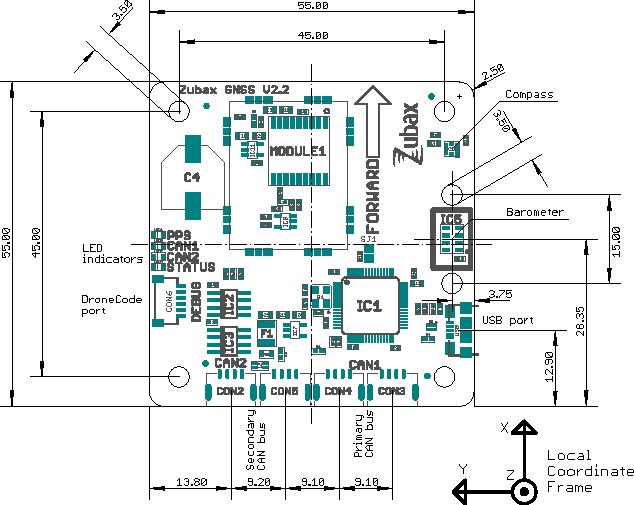
\includegraphics[width=1\textwidth]{GNSS2_drawing}
	\caption{GNSS2 drawing.\label{drawing}}
\end{figure}


\end{document}
